\section{Resultados}

	Como afirmado anteriormente, o primeiro passo do projeto é a prototipagem do Hardware do sistema, que inclui o Arduino, os botões e potenciômetros, através da plataforma online TinkerCAD, que inclui em si um monitor serial para visualizar o que está sendo enviado serialmente pelo microcontrolador.

\begin{figure}[htbp]
     \centerline{
        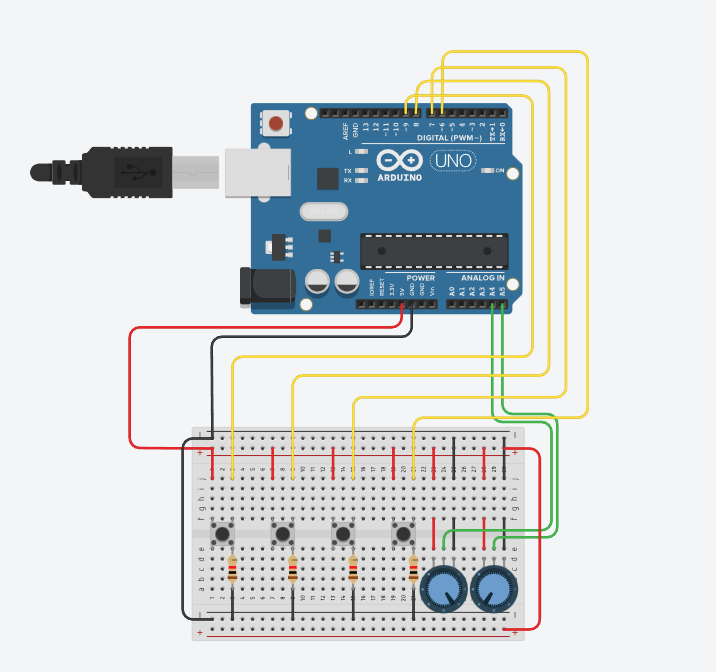
\includegraphics[width=3in]{tinkercad.png}
        }
     \caption{Modelo prototipado no TinkerCAD.}
     \label{fig}
    \end{figure}

	Como pode ser visto na figura acima, o modelo foi criado para abrigar dois potenciômetros e uma quantidade de botões, que foram 4 no momento da simulação. Cada um destes associados a um pino digital respectivo. Assim, a função do Arduino será pegar as informações desses componentes eletrônicos e enviar serialmente para o computador serialmente. O que tornará isso possível é a utilização da biblioteca "softwareserial.h" e suas funções, que possibilitam a comunicação.
	
	Para enviar todas as informações de uma única vez, em um pacote só, elas serão inseridas em uma string, e sua separação será realizada no código do Processing. Assim sendo, o código inserido no Arduino compreende a seguinte lógica:

\begin{lstlisting}[language=C]
const int pot1 = A5, pot2 = A3; //Potenciometros
const int b01 = 8, b02 = 7; // Botoes
int v_pot1 = 0, v_pot2 = 0; //Valores dos potenciometros
bool v_b01,v_b02; //Valores dos Botoes
int arr[10];

void setup() {
  Serial.begin(9600);
  pinMode(pot1, INPUT);
  pinMode(pot2, INPUT);
  
  for(int i = 7; i <= 8; i++){
      pinMode(i, INPUT_PULLUP);
    }
}

void loop() {
  v_pot1 = map(analogRead(pot1),0,1023,0,255);
  Serial.print(String(v_pot1) + "-");
  
  v_pot2 = map(analogRead(pot2),0,1023,0,255);
  Serial.print(String(v_pot2) + "-");
  
  v_b01 = !digitalRead(b01);
  v_b02 = !digitalRead(b02);

  Serial.print(String(v_b01) + "-");
  Serial.print(String(v_b02) + "\n");
  delay(50);
}
\end{lstlisting}

	%% explicação do código

	%% falar dos controles impressos 3D

	%% código no processing

	%% foto do Jogo



